\subsection{Aim}
To determine the standard molar enthalpy of formation of Magnesium Oxide (MgO).
\subsection{Materials Required}
Calorimeter, thermometer, Bunsen Burner, Beaker, Tongs, Electric Balance.
\subsection{Chemicals Required}
Magnesium Ribbon, HCl (1.0 M), NaOH (1.0M)

\subsection{Theory}
The \emph{standard enthalpy of formation} of a compound is the change of enthalpy during the formation of 1 mole of the substance from its constituent elements, with all substances in their standard states, and at a pressure of 1 bar.
\\ \\
The standard enthalpy of formation of Magnesium Oxide, would be the enthalpy of the reaction below:
\[ 
  \ce{Mg + 1/2O2 -> MgO} \tag{1}\label{1}
 \]
 \\
Reaction (1) releases a lot of heat and light energy, and a direct method for measuring this energy would be extremely difficult in an experimental environment. Thus, we utilize Hess’ Law to indirectly measure the enthalpy of this reaction.
 \\ \\
\emph{Hess' law} states that the total enthalpy change during the complete course of a chemical reaction is the same whether the reaction is made in one step or in several steps.
 \\ \\
Since it is easier and more accurate to measure the temperature change of a solution, we conduct the following reactions and measure the $\Delta T$ for each.
\cleardoublepage

\begin{align*}
\ce{& Mg(s) + 2H+(aq) -> Mg2+(aq) + H2(g)} \tag{2}\label{2} \\ \\
\ce{& MgO(s)  + 2H+(aq) ->  Mg2+(aq) + H2O(l)} \tag{3}\label{3} \\ \\
\ce{& 1/2O2(g) + H2(g) -> H2O(l)} \tag{4}\label{4} \\ \\
\end{align*}
We can clearly see that (2) - (3) + (4) = (1), thus the reactions can be used to determine the $\Delta H$ of formation of MgO. Note that reaction (4) is a standard reaction whose $\Delta H$ is known to be approximately 285.8 kJ/mol.
 \\ \\
To measure $\Delta T$ for each reaction accurately, we conduct each reaction in a calorimeter, to prevent any loss of heat to the surroundings and thus minimize error. As reactions are carried out in a constant pressure environment, the heat released is equal to the enthalpy change in the reaction
\\ \\
In a solution of n moles, for a change in temp of $\Delta T$, the heat released $Q$ is given by:
\[
  Q = nC\Delta T \tag{5}\label{5}
\]
Where C is the molar heat capacity of the medium/body where change of temperature occurs.
\\ \\
In this experiment,we need to first determine the $C$ of the calorimeter, as this value is unknown to us. For this, we conduct the following reaction separately in the calorimeter and measure the change in temperature $\Delta T_1$:
\begin{align*}
\ce{nNaOH(1M) + nHCL(1M) -> nNaCl + nH2O} \tag{6}\label{6}
\end{align*}

The $\Delta H$ for this reaction is known to be -55.8 kJ/mol.
\\
Also,
\[
  \text{Moles of water in the solution}(n^\prime)  = \frac{2n}{18}
\]
\\
We also know that,
\begin{align*}
&\text{Heat absorbed by calorimeter}(Q_{cal}) = \text{Heat released by reaction} - \text{Heat absorbed by Water} \\ \\
\implies & Q_{cal} = (-55800J \times n) - (\text{Moles of water in solution} \times 75.348 J/mol K \times \Delta T_1)
\end{align*}
Thus, the heat capacity of the calorimeter is,
\[
  C_{cal}=\frac{Q_{cal}}{\Delta T_1} \tag{7}\label{7}
\]
\\
After this value is known to use, we can use (5) to calculate the $\Delta H$ for reactions (1) to (4), and thus compute the enthalpy of formation of MgO.
\cleartoleftpage
\vspace*{6cm}
\begin{figure}[h]
  \begin{center}
    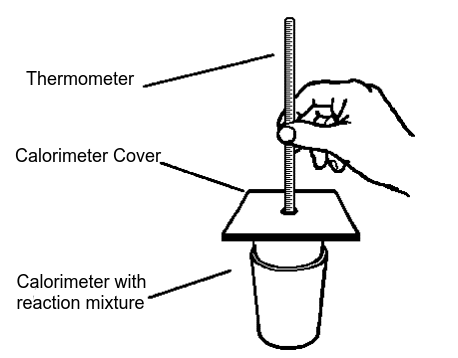
\includegraphics[width=10cm]{fig2}
    \end{center}
  \caption*{Fig.2 Experimental Setup for measuring temperature changes in reactions}
 \end{figure}
\cleardoublepage
\subsection{Procedure}
Determining Heat capacity of Calorimeter:
\begin{enumerate}
\item To determine heat capacity of calorimeter, the reaction between HCL and NaOH is carried out in aqueous solution in calorimeter.
\item Prepare standard solutions of 1M HCl by diluting 12M HCl and 1M NaOH by dissolving 40g NaOH pellets in 100 ml of  water in standard flasks.
\item Take a calorimeter and place a thermometer in it. Note the initial reading of thermometer.
\item Add 15ml each of standard HCl and NaOH in the calorimeter.
\item Keep observing the thermometer until its temperature reaches a maximum value. Note the reading.
\item Calculate the value of heat capacity of the calorimeter.
\end{enumerate}
\vspace{5mm}
Measuring enthalpy of formation of MgO:
\begin{enumerate}
\item Weigh 0.3g(0.025 mol) of Mg on an electronic balance.
\item Take the same calorimeter whose heat capacity was determined and add the 0.3g of Mg to it.
\item Take a thermometer and place it in the calorimeter. Note the initial reading of thermometer.
\item Add 25ml of standard HCl solution(1M) to the calorimeter. Note the maximum temperature of the thermometer.
\item Burn some Mg ribbons and take 0.5g(0.025 mol) of the MgO formed.
\item Wash the calorimeter and add the MgO to it. 
\item Take a thermometer and place it in the calorimeter. Note the initial reading of thermometer.
\item Add 25ml of standard HCl solution(1M) to the calorimeter. Note the maximum temperature of the thermometer.
\item Use the obtained readings to calculate enthalpies of the above reactions per mole of HCl and hence determine the enthalpy of formation of MgO.
\end{enumerate}

\cleardoublepage
\subsection{Observations}
Temperature change for HCl + NaOH reaction $(\Delta T_1) = \text{Final - Inital} = 32.5 - 29 = 3.5\degree C$ \\
Temperature change for Mg+HCl reaction $(\Delta T_2) = \text{Final - Inital} = 58 - 25 = 33\degree C$ \\
Temperature change for MgO+HCl reaction $(\Delta T_3) = \text{Final - Inital} = 36 - 31 = 5\degree C$ \\

\subsection{Calculations}
Calculating Heat Capacity of Calorimeter:
By Equation (7) in Theory,
\begin{align*}
  C_{cal}&=\frac{(55800J/molK * 0.015 mol) - (\frac{30}{18} mol * 75.348J/mol K * 3.5\degree C)}{3.5\degree C} \\
  &= \frac{397.47}{3.5} \\
    \implies C_{cal}&=113.56 J/K
\end{align*}
\\
Since in the reactions of Mg with HCl and MgO with HCl, the solution had the same quantity of water (25 ml), thus we can include the heat absorbed by this water in our calorimeter's heat capacity, thus obtaining its \emph{Effective Heat Capacity} ($C_{eff}$). Note that this is done purely for ease of calculation in subsequent steps.
\begin{align*}
  C_{eff} &= (\frac{25}{18} \times 75.348) + 113.56 \\
  &=218.21 J/K \\
\end{align*}

Thus, enthalpy change for Mg + HCl reaction $(H_1)$ and for MgO + HCl $(H_2)$ is given by:
\begin{align*}
  \Delta H_1 &= \frac{33*218.21}{0.025} = 288.03 KJ/mol \\ \\
  \Delta H_2 &= \frac{5*218.21}{0.025} = 43.642 KJ/mol
\end{align*}

Thus the enthalpy of formation of MgO within experimental errors is:
\begin{align*}
  \Delta H_f &= 285.8 + 288.03 - 43.642 \\
&= 530.19 kJ/mol
\end{align*}

\subsection{Result}
Known Standard Enthalpy of Formation of MgO is \textbf{601.8 kJ/mol}. \\
Calculated Standard Enthalpy of Formation of MgO is \textbf{530.2 kJ/mol} \\
Percentage Error = 12\%
\subsection{Precautions}
\begin{enumerate}
\item Burn the magnesium ribbon carefully, holding the reactant with tongs away from face.
  \cleardoublepage
\item Handle Bunsen burner Carefully
\item Ensure to Cover Calorimeter to prevent heat loss
\item Avoid any parallax while taking temperature readings from the thermometer.
  \item Wash all apparatus thouroughly before pouring in any reactant.
\end{enumerate}


                                                                           
%%% Local Variables:
%%% mode: latex
%%% TeX-master: "../experiment"
%%% End:
